\documentclass[envcountsect,dvips]{beamer}

\setbeamertemplate{background canvas}[vertical shading][bottom=yellow!20,top=blue!10]
%\usetheme{Darmstadt}
\usetheme{Warsaw}
%\usefonttheme[onlysmall]{structurebold}

\usepackage{natbib}
\usepackage{bibentry}
\bibliographystyle{plain}
\usepackage{chngcntr}

\usepackage[utf8]{inputenc}
\usepackage{default}
\usepackage{amsmath}
\usepackage{amsfonts}
\usepackage{amssymb}

\usepackage{graphicx}
\usepackage{caption}
\usepackage{subcaption}

\usepackage{color,xcolor,ucs}% para textcolor

%%%%%%%%%%%%%%%%%%%%%%%%%%%%%%%%%%%%%%%%%%%%%%%%%%%%%%%%%%%%%%%%%%%%%%%%%%
%%%%%%%%%%%%%%%%%%%%%%%%%%%%%%%%%%%%%%%%%%%%%%%%%%%%%%%%%%%%%%%%%%%%%%%%%%
%%%%%%%%%%%%%%%%%%%%%%%%%%%%%%%%%%%%%%%%%%%%%%%%%%%%%%%%%%%%%%%%%%%%%%%%%%
%%%%%%%%%%%%%%%%%%%%%%%%%%%%%%%%%%%%%%%%%%%%%%%%%%%%%%%%%%%%%%%%%%%%%%%%%%

\definecolor{dkred}{rgb}{0.6,0,0}
\definecolor{dkgreen}{rgb}{0,0.6,0}
\definecolor{dkblue}{rgb}{0,0,0.6}
\definecolor{mygray}{rgb}{0.5,0.5,0.5}
\definecolor{mylowgray}{rgb}{0.9,0.9,0.9}
\definecolor{myverylowgray}{rgb}{0.95,0.95,0.95}
\definecolor{mymauve}{rgb}{0.58,0,0.82}
\definecolor{lavender}{rgb}{1.00,0.94,0.96}


%%%%%%%%%%%%%%%%%%%%%%%%%%%%%%%%%%%%%%%%%%%%%%%%%%%%%%%%%%%%%%%%%%%%%%%%%%
%show only the current section in the head
\setbeamertemplate{headline}
{%
  \leavevmode%
  \begin{beamercolorbox}[wd=.5\paperwidth,ht=2.5ex,dp=1.125ex]{section in head/foot}%
    \hbox to .5\paperwidth{\hfil\insertsectionhead\hfil}
  \end{beamercolorbox}%
  \begin{beamercolorbox}[wd=.5\paperwidth,ht=2.5ex,dp=1.125ex]{subsection in head/foot}%
    \hbox to .5\paperwidth{\hfil\insertsubsectionhead\hfil}
  \end{beamercolorbox}%
}


%%%%%%%%%%%%%%%%%%%%%%%%%%%%%%%%%%%%%%%%%%%%%%%%%%%%%%%%%%%%%%%%%%%%%%%%%%
\AtBeginSection[]{
  \begin{frame}
  \vfill
  \centering
  \begin{beamercolorbox}[sep=8pt,center,shadow=true,rounded=true]{title}
    \usebeamerfont{title}\insertsectionhead\par%
  \end{beamercolorbox}
  \vfill
  \end{frame}
}

%%%%%%%%%%%%%%%%%%%%%%%%%%%%%%%%%%%%%%%%%%%%%%%%%%%%%%%%%%%%%%%%%%%%%%%%%%
%%%%%%%%%%%%%%%%%%%%%%%%%%%%%%%%%%%%%%%%%%%%%%%%%%%%%%%%%%%%%%%%%%%%%%%%%%
%%%%%%%%%%%%%%%%%%%%%%%%%%%%%%%%%%%%%%%%%%%%%%%%%%%%%%%%%%%%%%%%%%%%%%%%%%
%%%%%%%%%%%%%%%%%%%%%%%%%%%%%%%%%%%%%%%%%%%%%%%%%%%%%%%%%%%%%%%%%%%%%%%%%%
\newenvironment<>{varblock}[2][.9\textwidth]{%
  \setlength{\textwidth}{#1}
  \begin{actionenv}#3%
    \def\insertblocktitle{#2}%
    \par%
    \usebeamertemplate{block begin}}
  {\par%
    \usebeamertemplate{block end}%
  \end{actionenv}}

%%%%%%%%%%%%%%%%%%%%%%%%%%%%%%%%%%%%%%%%%%%%%%%%%%%%%%%%%%%%%%%%%%%%%%%%%%
\begin{document}

\title[Aritmética com inteiros:   ] % (optional, only for long titles)
{TEMAS DE PESQUISA NO DESENVOLVIMENTO DE INSTRUMENTAÇÃO E PROCESSAMENTO DIGITAL DE SINAIS }
\subtitle{EM ENGENHARIA APLICADA}
\author[Fernando] % (optional, for multiple authors)
{Fernando Pujaico Rivera\inst{1}}
\institute[Universidade Federal de Lavras] % (optional)
{
  \inst{1}%
  Universidade Federal de Lavras
}
\date[2018] % (optional)
{2018}
\subject{Computer Science}
\frame{\titlepage}

%%%%%%%%%%%%%%%%%%%%%%%%%%%%%%%%%%%%%%%%%%%%%%%%%%%%%%%%%%%%%%%%%%%%%%%%%%%%%%%%
%%%%%%%%%%%%%%%%%%%%%%%%%%%%%%%%%%%%%%%%%%%%%%%%%%%%%%%%%%%%%%%%%%%%%%%%%%%%%%%%
%%%%%%%%%%%%%%%%%%%%%%%%%%%%%%%%%%%%%%%%%%%%%%%%%%%%%%%%%%%%%%%%%%%%%%%%%%%%%%%%
\section{PDS Project Library: Linguagem C }
%%%%%%%%%%%%%%%%%%%%%%%%%%%%%%%%%%%%%%%%%%%%%%%%%%%%%%%%%%%%%%%%%%%%%%%%%%%%%%%%%

%%%%%%%%%%%%%%%%%%%%%%%%%%%%%%%%%%%%%%%%%%%%%%%%%%%%%%%%%%%%%%%%%%%%%%%%%%%%%%%%%
\begin{frame}{http://www.nongnu.org/pdsplibrary/}
\begin{center}
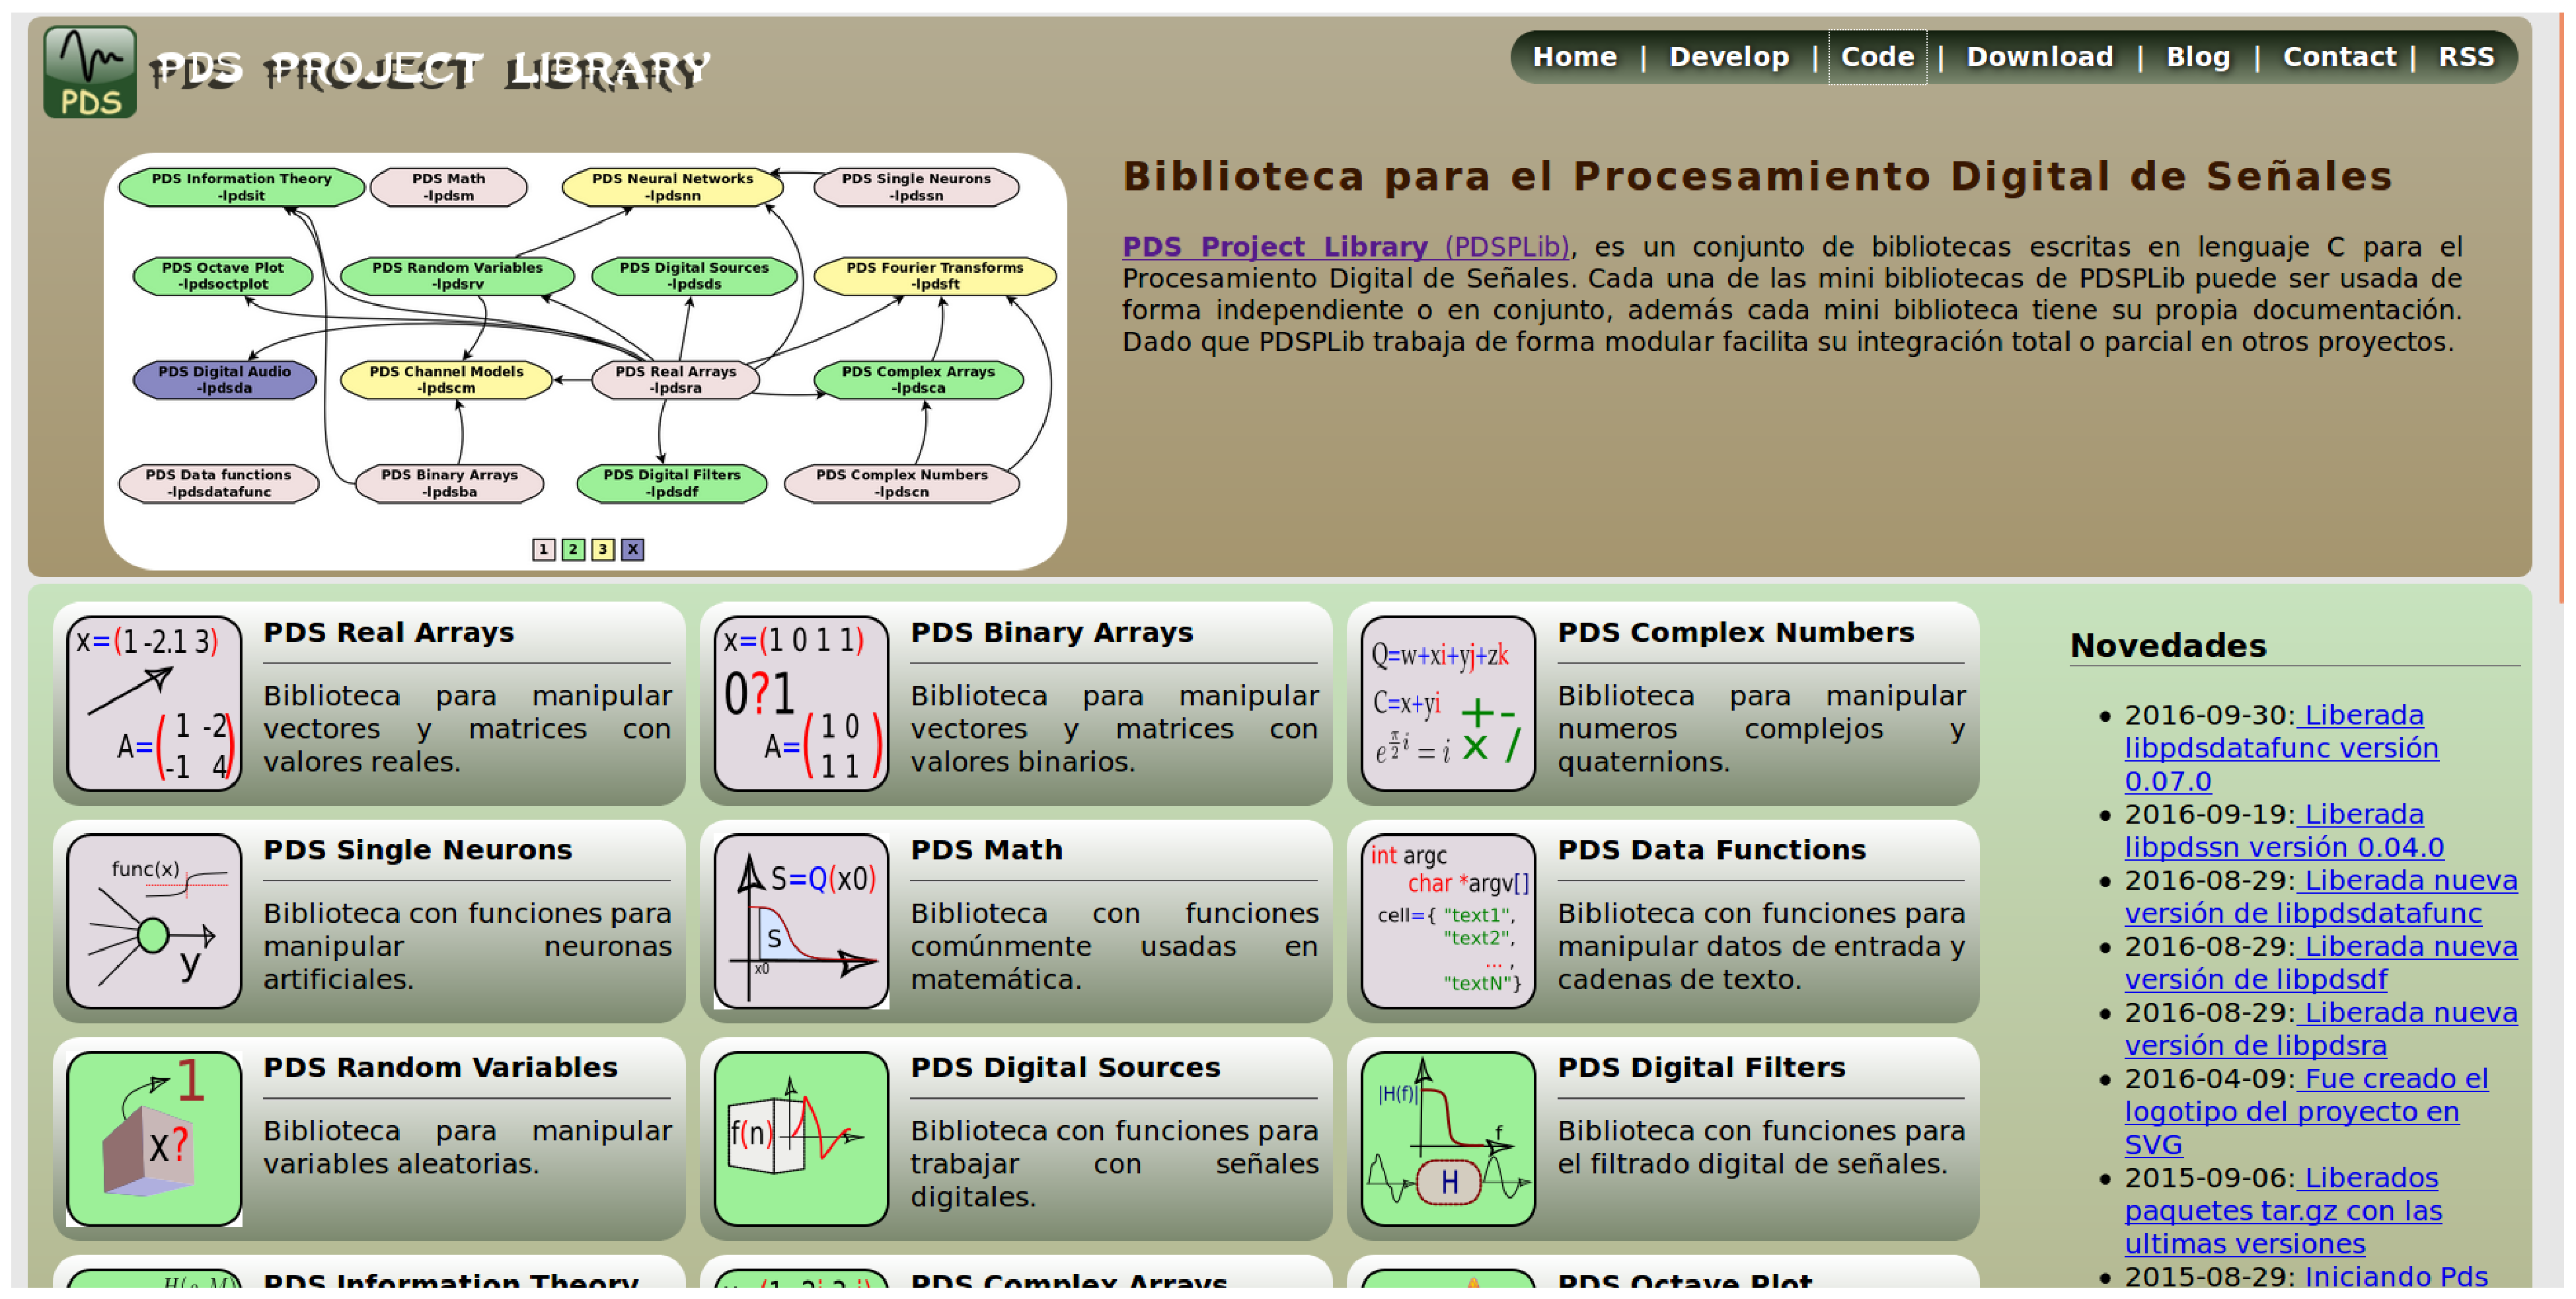
\includegraphics[width=\textwidth]{images/pdsplibrary.eps}
\end{center} 
\end{frame}


%%%%%%%%%%%%%%%%%%%%%%%%%%%%%%%%%%%%%%%%%%%%%%%%%%%%%%%%%%%%%%%%%%%%%%%%%%%%%%%%%
\begin{frame}{http://www.nongnu.org/pdsplibrary/}
\begin{center}
\begin{figure}
    \centering
    \begin{subfigure}[b]{0.25\textwidth}
        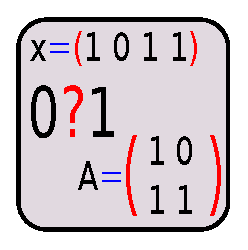
\includegraphics[width=\textwidth]{images/libpdsba.eps}
        \caption{libpdsba}
        \label{fig:libpdsba}
    \end{subfigure}
    \begin{subfigure}[b]{0.25\textwidth}
        \includegraphics[width=\textwidth]{images/libpdsca.eps}
        \caption{libpdsca}
        \label{fig:libpdsca}
    \end{subfigure}
    \begin{subfigure}[b]{0.25\textwidth}
        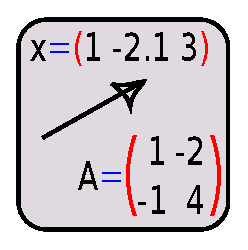
\includegraphics[width=\textwidth]{images/libpdsra.eps}
        \caption{libpdsra}
        \label{fig:libpdsra}
    \end{subfigure}
    \begin{subfigure}[b]{0.25\textwidth}
        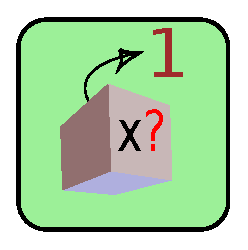
\includegraphics[width=\textwidth]{images/libpdsrv.eps}
        \caption{libpdsrv}
        \label{fig:libpdsrv}
    \end{subfigure}
    \begin{subfigure}[b]{0.25\textwidth}
        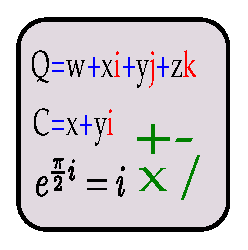
\includegraphics[width=\textwidth]{images/libpdscn.eps}
        \caption{libpdscn}
        \label{fig:libpdscn}
    \end{subfigure}
    \begin{subfigure}[b]{0.25\textwidth}
        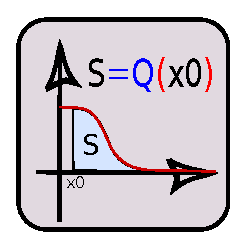
\includegraphics[width=\textwidth]{images/libpdsm.eps}
        \caption{libpdsm}
        \label{fig:libpdsm}
    \end{subfigure}
    \caption{Bibliotecas em C para o projeto PDS }\label{fig:animals}
\end{figure}
\end{center}

\end{frame}

%%%%%%%%%%%%%%%%%%%%%%%%%%%%%%%%%%%%%%%%%%%%%%%%%%%%%%%%%%%%%%%%%%%%%%%%%%%%%%%%%
\begin{frame}{http://www.nongnu.org/pdsplibrary/}
\begin{center}
\begin{figure}
    \centering
    \begin{subfigure}[b]{0.25\textwidth}
        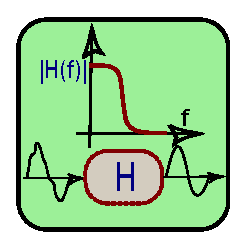
\includegraphics[width=\textwidth]{images/libpdsdf.eps}
        \caption{libpdsdf}
        \label{fig:libpdsdf}
    \end{subfigure}
    \begin{subfigure}[b]{0.25\textwidth}
        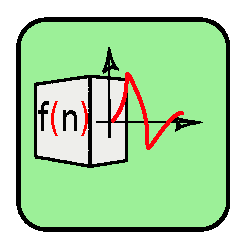
\includegraphics[width=\textwidth]{images/libpdsds.eps}
        \caption{libpdsds}
        \label{fig:libpdsds}
    \end{subfigure}
    \begin{subfigure}[b]{0.25\textwidth}
        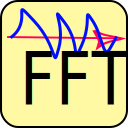
\includegraphics[width=\textwidth]{images/libpdsft.eps}
        \caption{libpdsft}
        \label{fig:libpdsft}
    \end{subfigure}
    \begin{subfigure}[b]{0.25\textwidth}
        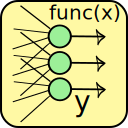
\includegraphics[width=\textwidth]{images/libpdsnn.eps}
        \caption{libpdsnn}
        \label{fig:libpdsnn}
    \end{subfigure}
    \begin{subfigure}[b]{0.25\textwidth}
        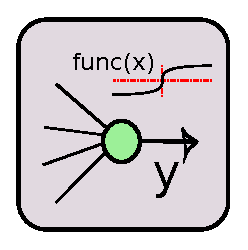
\includegraphics[width=\textwidth]{images/libpdssn.eps}
        \caption{libpdssn}
        \label{fig:libpdssn}
    \end{subfigure}
    \begin{subfigure}[b]{0.25\textwidth}
        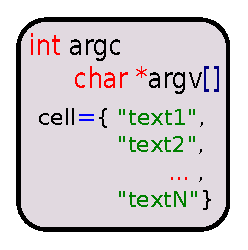
\includegraphics[width=\textwidth]{images/libpdsdatafunc.eps}
        \caption{libpdsdatafunc}
        \label{fig:libpdsdatafunc}
    \end{subfigure}
    \caption{Bibliotecas em C para o projeto PDS }\label{fig:animals}
\end{figure}
\end{center}
\end{frame}


%%%%%%%%%%%%%%%%%%%%%%%%%%%%%%%%%%%%%%%%%%%%%%%%%%%%%%%%%%%%%%%%%%%%%%%%%%%%%%%%
%%%%%%%%%%%%%%%%%%%%%%%%%%%%%%%%%%%%%%%%%%%%%%%%%%%%%%%%%%%%%%%%%%%%%%%%%%%%%%%%
%%%%%%%%%%%%%%%%%%%%%%%%%%%%%%%%%%%%%%%%%%%%%%%%%%%%%%%%%%%%%%%%%%%%%%%%%%%%%%%%
\section{PDS Project Library: Linguagem Java }
%%%%%%%%%%%%%%%%%%%%%%%%%%%%%%%%%%%%%%%%%%%%%%%%%%%%%%%%%%%%%%%%%%%%%%%%%%%%%%%%%

%%%%%%%%%%%%%%%%%%%%%%%%%%%%%%%%%%%%%%%%%%%%%%%%%%%%%%%%%%%%%%%%%%%%%%%%%%%%%%%%%
\begin{frame}{https://sourceforge.net/projects/pdsplibj/}
\begin{center}
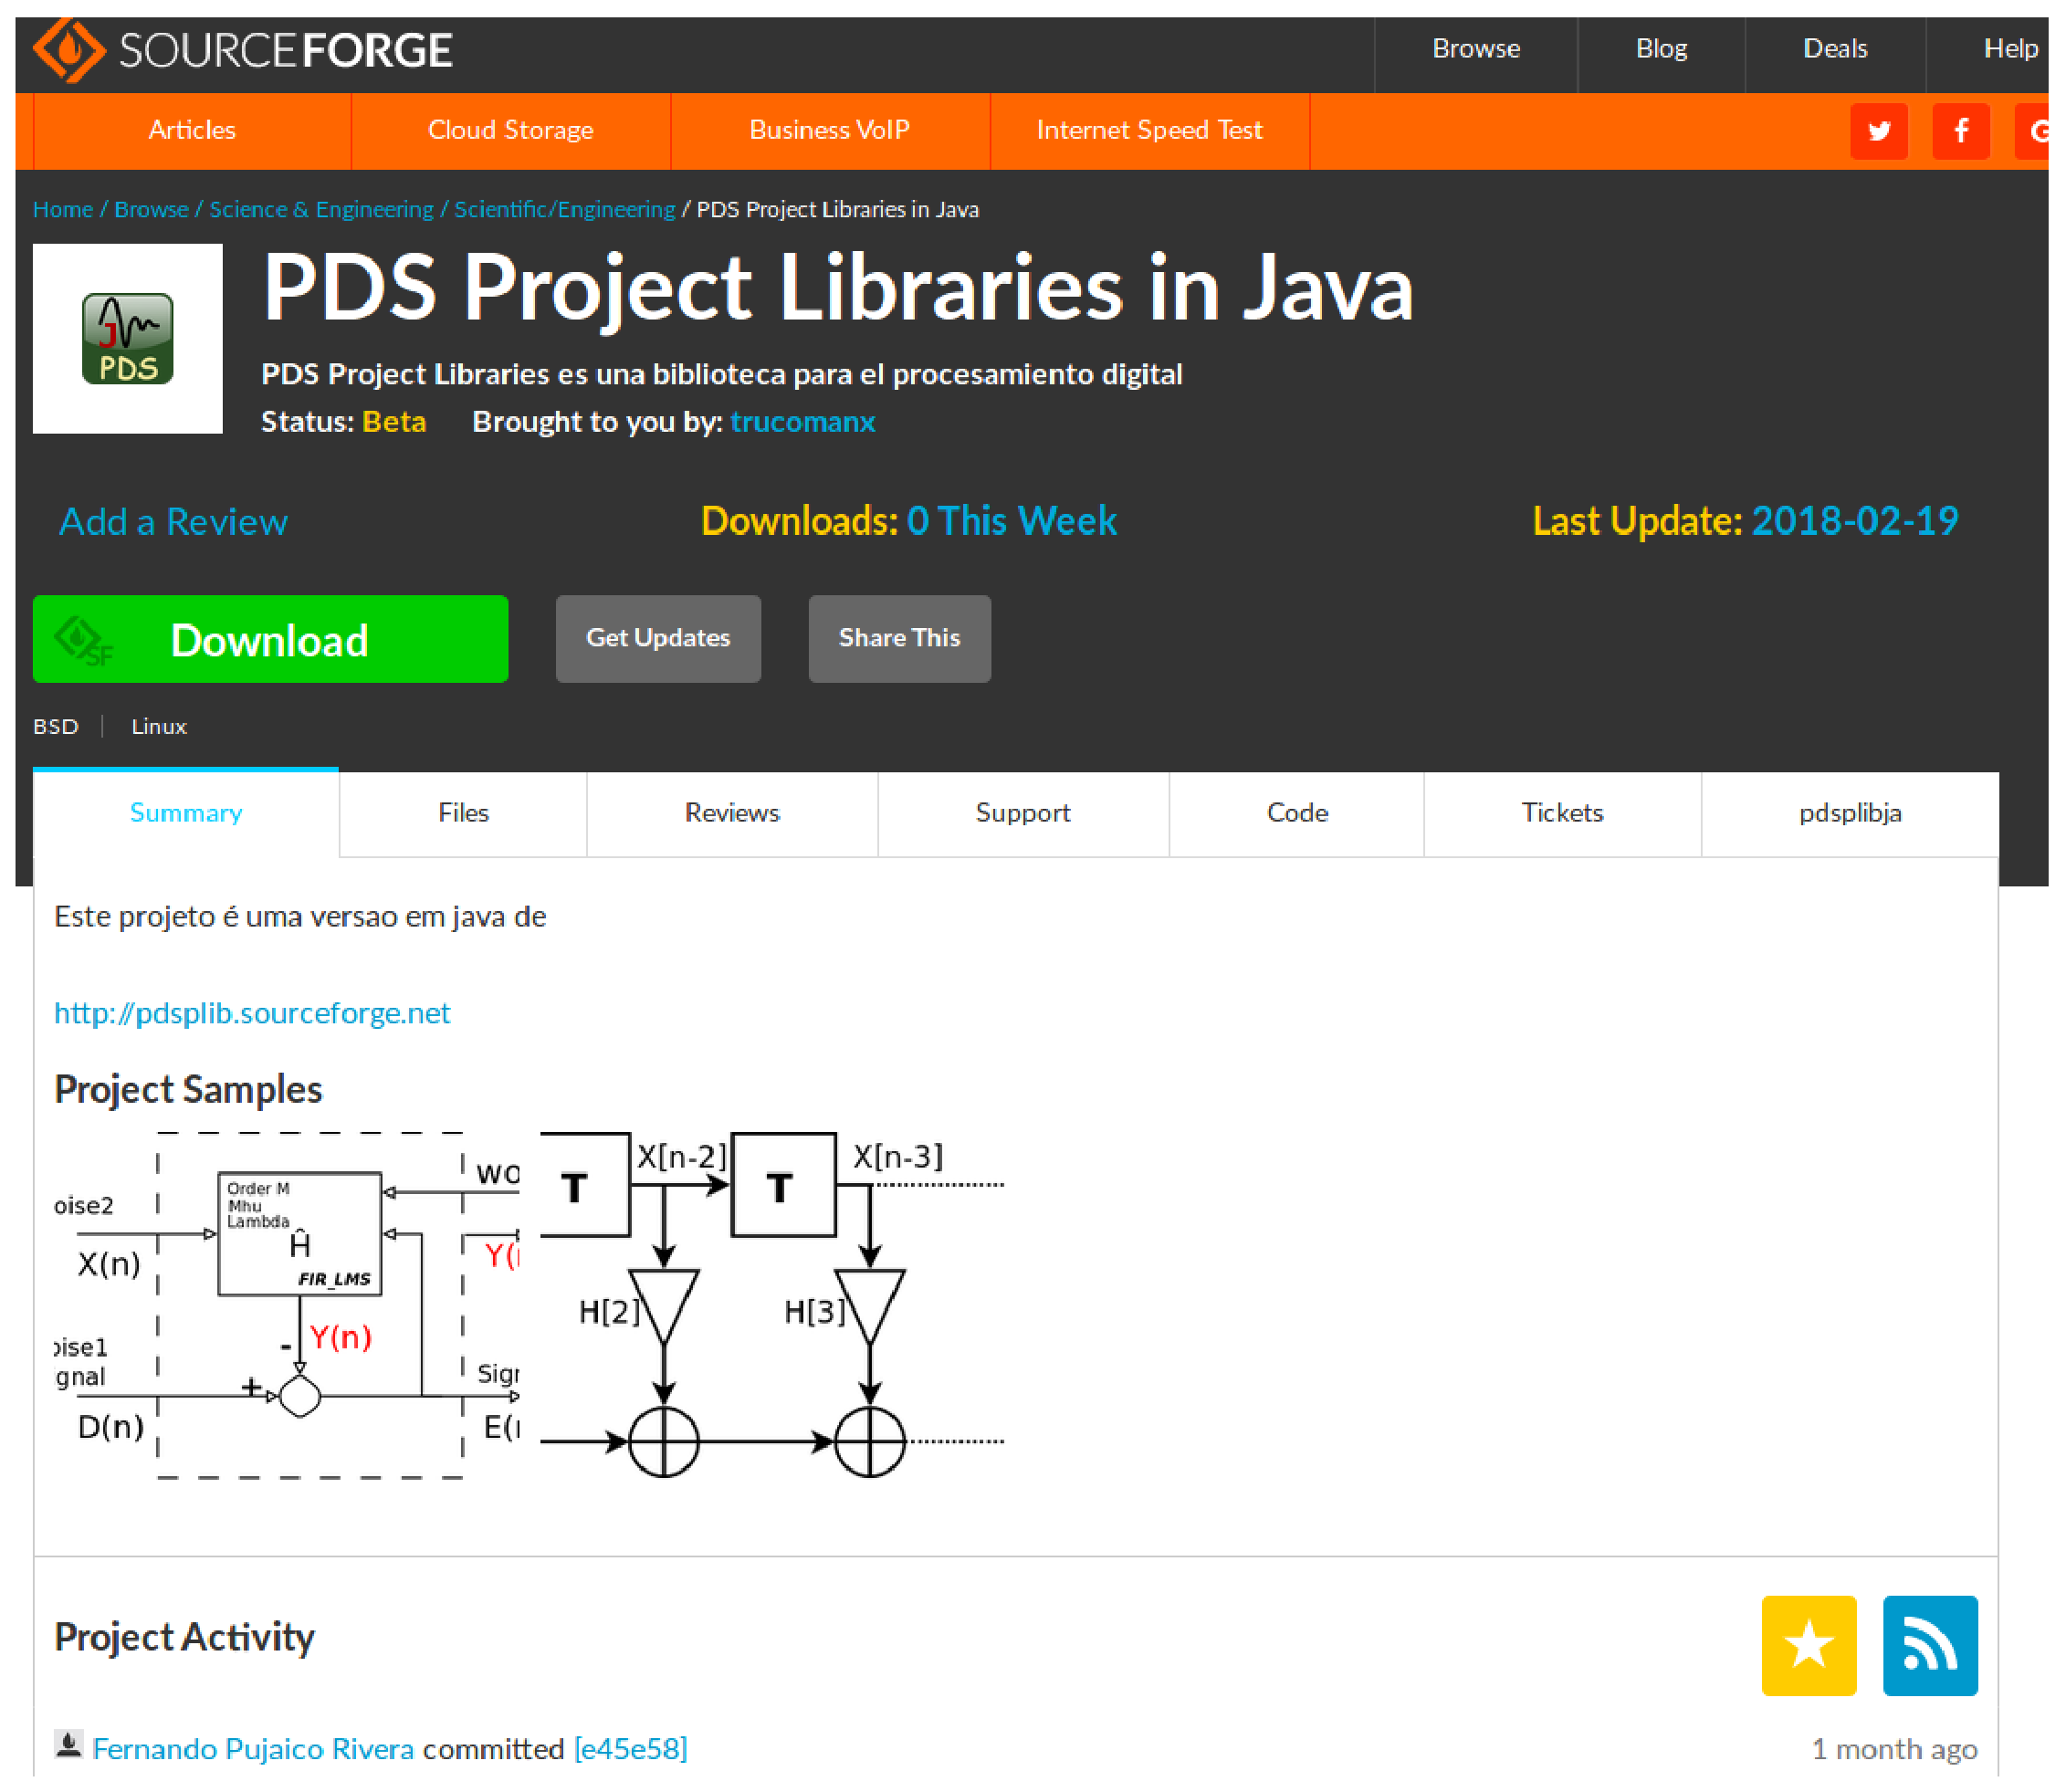
\includegraphics[width=\textwidth]{images/pdsplibraryj.eps}
\end{center} 
\end{frame}

%%%%%%%%%%%%%%%%%%%%%%%%%%%%%%%%%%%%%%%%%%%%%%%%%%%%%%%%%%%%%%%%%%%%%%%%%%%%%%%%%
\begin{frame}{https://sourceforge.net/projects/pdsplibj/}
\begin{center}
\begin{figure}
    \centering
    \begin{subfigure}[b]{0.25\textwidth}
        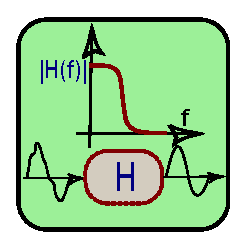
\includegraphics[width=\textwidth]{images/libpdsdf.eps}
        \caption{pdsdf}
        \label{fig:pdsdf}
    \end{subfigure}
    \begin{subfigure}[b]{0.25\textwidth}
        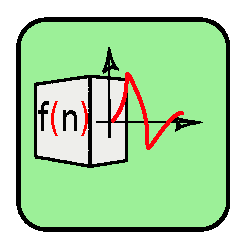
\includegraphics[width=\textwidth]{images/libpdsds.eps}
        \caption{pdsds}
        \label{fig:pdsca}
    \end{subfigure}
    ~\\
    \begin{subfigure}[b]{0.25\textwidth}
        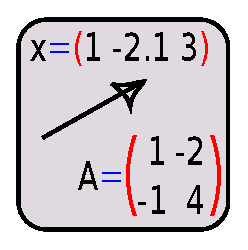
\includegraphics[width=\textwidth]{images/libpdsra.eps}
        \caption{pdsra}
        \label{fig:pdsra}
    \end{subfigure}
    \begin{subfigure}[b]{0.25\textwidth}
        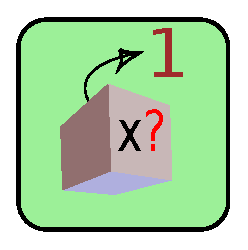
\includegraphics[width=\textwidth]{images/libpdsrv.eps}
        \caption{pdsrv}
        \label{fig:pdsrv}
    \end{subfigure}
    \caption{Bibliotecas em C para o projeto PDS }\label{fig:animals}
\end{figure}
\end{center}

\end{frame}

%%%%%%%%%%%%%%%%%%%%%%%%%%%%%%%%%%%%%%%%%%%%%%%%%%%%%%%%%%%%%%%%%%%%%%%%%%%%%%%%%
%%%%%%%%%%%%%%%%%%%%%%%%%%%%%%%%%%%%%%%%%%%%%%%%%%%%%%%%%%%%%%%%%%%%%%%%%%%%%%%%%
%%%%%%%%%%%%%%%%%%%%%%%%%%%%%%%%%%%%%%%%%%%%%%%%%%%%%%%%%%%%%%%%%%%%%%%%%%%%%%%%%
\section{PDS Project Library: Linguagem Java : Área foliar }
%%%%%%%%%%%%%%%%%%%%%%%%%%%%%%%%%%%%%%%%%%%%%%%%%%%%%%%%%%%%%%%%%%%%%%%%%%%%%%%%%

%%%%%%%%%%%%%%%%%%%%%%%%%%%%%%%%%%%%%%%%%%%%%%%%%%%%%%%%%%%%%%%%%%%%%%%%%%%%%%%%%
\begin{frame}{https://sourceforge.net/projects/pdsplibj/}
\begin{minipage}[c]{0.6\textwidth}
\begin{center}
\begin{figure}
    \centering
    \begin{subfigure}[b]{0.45\textwidth}
        \includegraphics[width=\textwidth]{images/img1.eps}
        \caption{Imagem original}
        \label{fig:pdsimg1}
    \end{subfigure}
    \begin{subfigure}[b]{0.45\textwidth}
        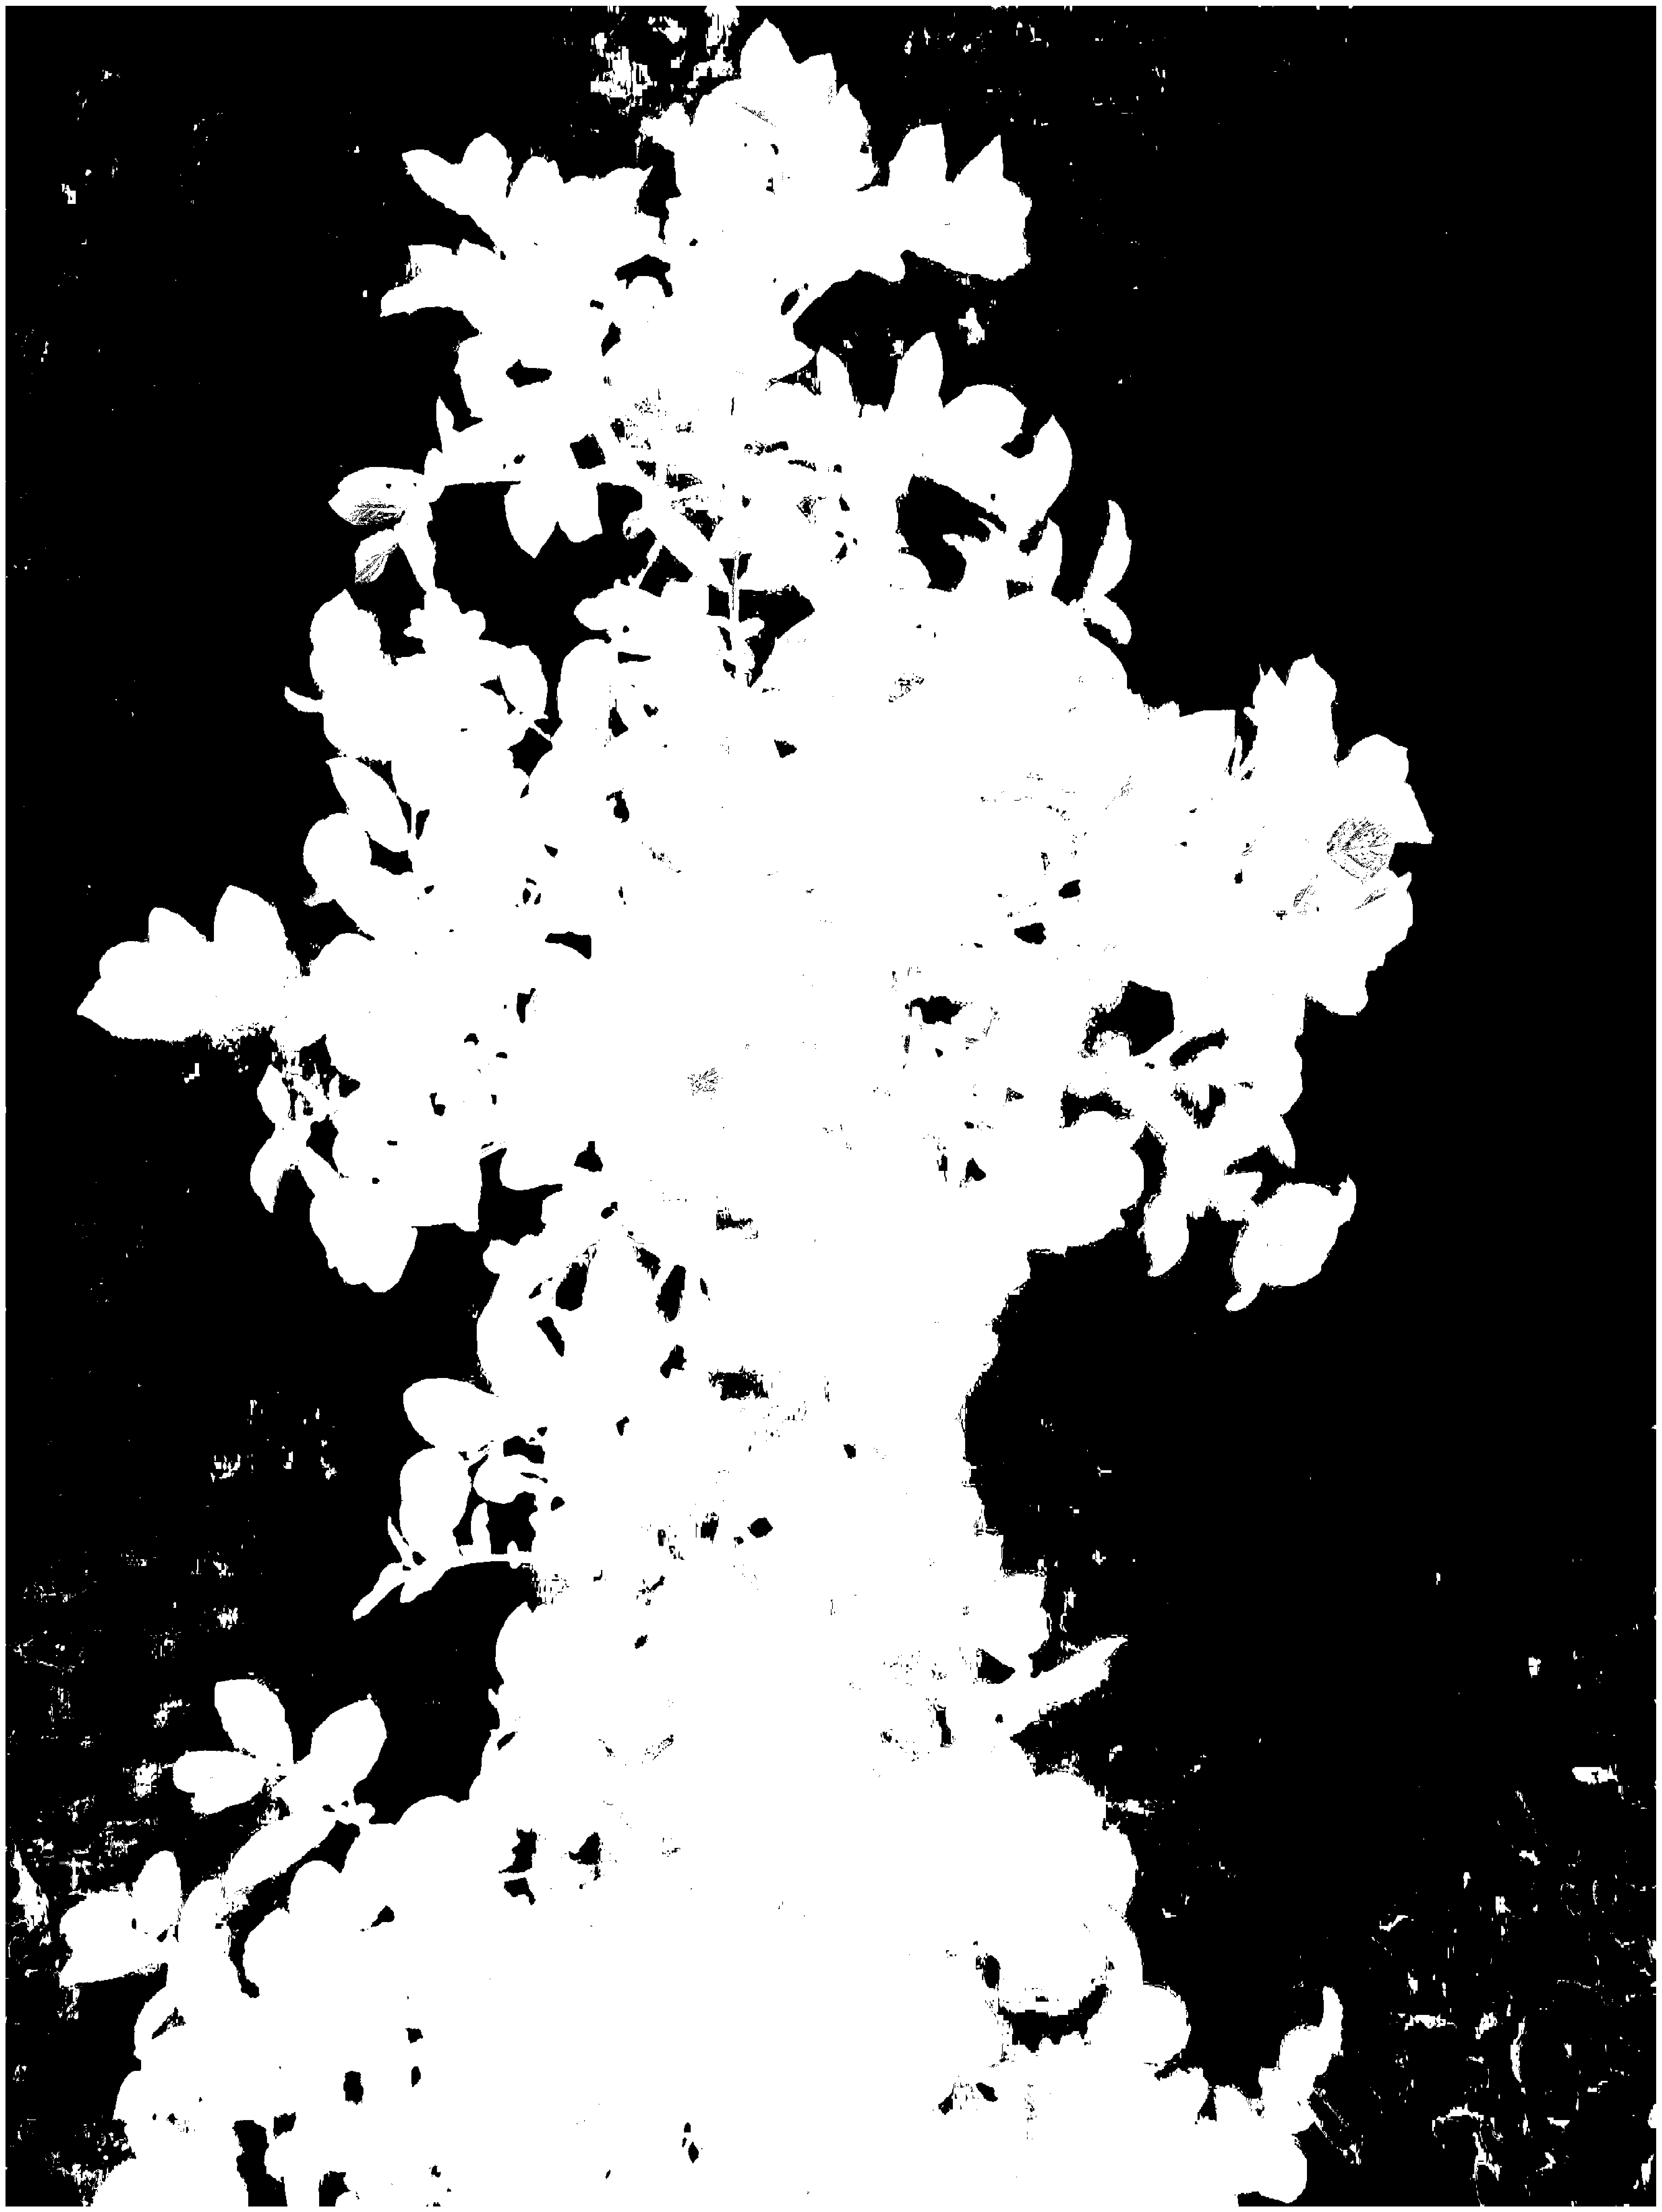
\includegraphics[width=\textwidth]{images/img1-1.eps}
        \caption{Imagem filtrada}
        \label{fig:pdsimg11}
    \end{subfigure}
    \caption{Bibliotecas em Java para o projeto PDS }\label{fig:PdsGcp}
\end{figure}
\end{center} 
\end{minipage}%
\begin{minipage}[c]{0.4\textwidth}
\begin{center}
 \textbf{PdsGcp}\\
Area foliar
\end{center}
A =  7990272\\
Agreen =  3554144\\
\end{minipage}
\end{frame}
%%%%%%%%%%%%%%%%%%%%%%%%%%%%%%%%%%%%%%%%%%%%%%%%%%%%%%%%%%%%%%%%%%%%%%%%%%%%%%%%%
\begin{frame}{https://sourceforge.net/projects/pdsplibj/}
\begin{minipage}[c]{0.6\textwidth}
\begin{center}
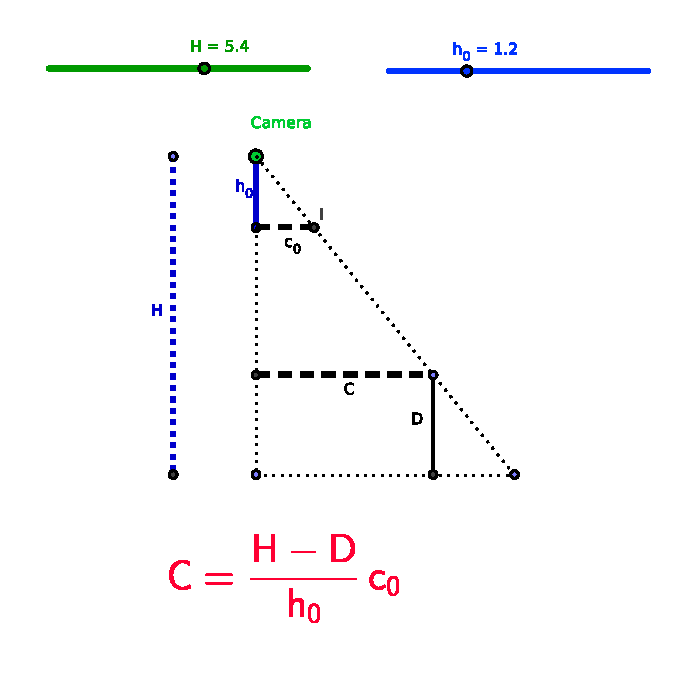
\includegraphics[width=1.0\textwidth]{images/vista2-problem.eps}
\end{center} 
\end{minipage}%
\begin{minipage}[c]{0.4\textwidth}
\begin{center}
 \textbf{PdsGcp}\\
Area foliar
\end{center}
A =  7990272\\
Agreen =  3554144\\
\end{minipage}
\end{frame}

%%%%%%%%%%%%%%%%%%%%%%%%%%%%%%%%%%%%%%%%%%%%%%%%%%%%%%%%%%%%%%%%%%%%%%%%%%%%%%%%%
%%%%%%%%%%%%%%%%%%%%%%%%%%%%%%%%%%%%%%%%%%%%%%%%%%%%%%%%%%%%%%%%%%%%%%%%%%%%%%%%%
%%%%%%%%%%%%%%%%%%%%%%%%%%%%%%%%%%%%%%%%%%%%%%%%%%%%%%%%%%%%%%%%%%%%%%%%%%%%%%%%%
\section{PDS Project Library: Linguagem Java : PIV }
%%%%%%%%%%%%%%%%%%%%%%%%%%%%%%%%%%%%%%%%%%%%%%%%%%%%%%%%%%%%%%%%%%%%%%%%%%%%%%%%%

%%%%%%%%%%%%%%%%%%%%%%%%%%%%%%%%%%%%%%%%%%%%%%%%%%%%%%%%%%%%%%%%%%%%%%%%%%%%%%%%%
\begin{frame}{https://sourceforge.net/projects/pdsplibj/}
\begin{minipage}[c]{0.6\textwidth}
\begin{center}
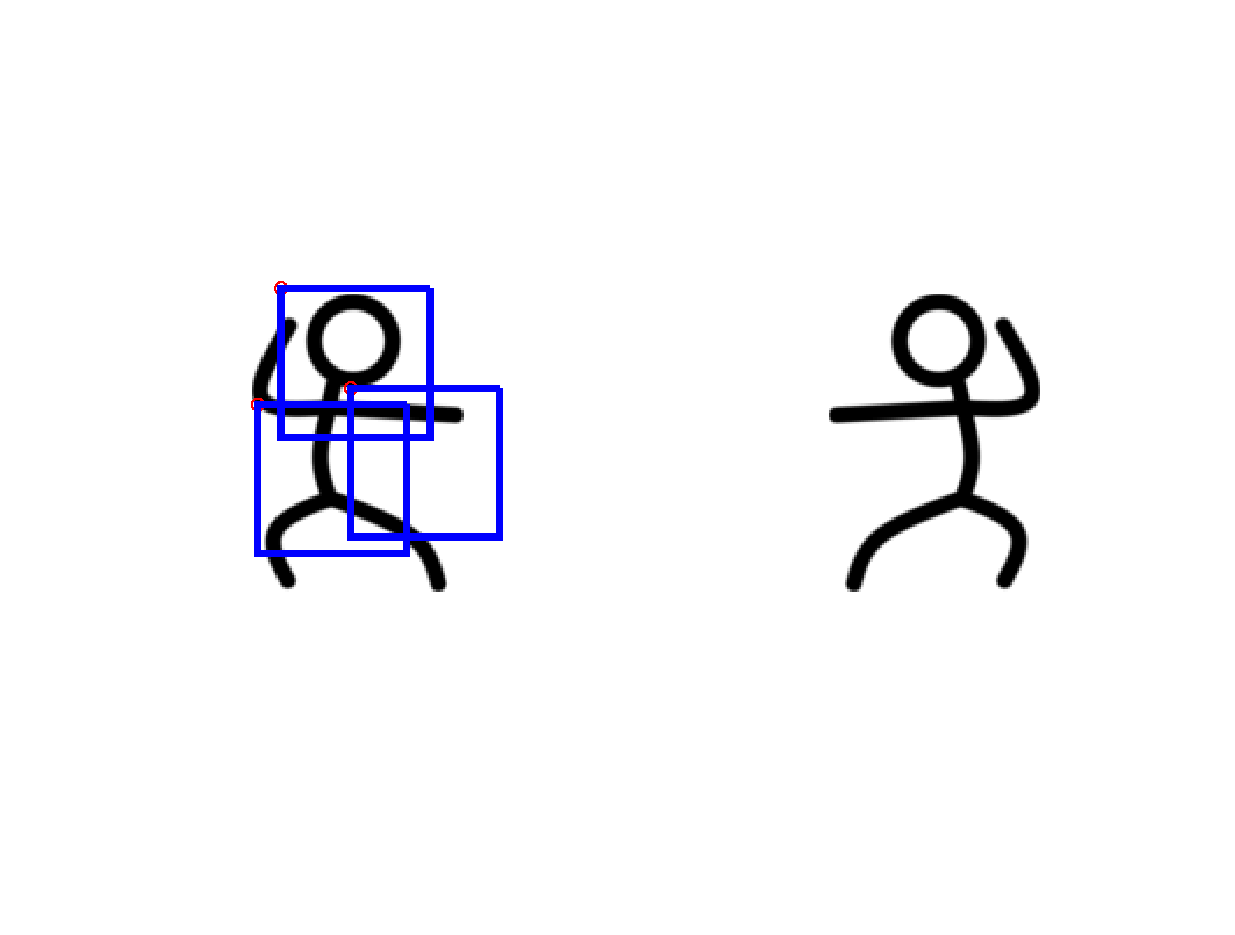
\includegraphics[width=1.0\textwidth]{images/1.eps}
\end{center} 
\end{minipage}%
\begin{minipage}[c]{0.4\textwidth}
\begin{center}
 \textbf{PdsPiv}\\
 Particle image velocimetry
\end{center}
\begin{equation*}
\rho = corr(\mathbf{A},\mathbf{X})
  \end{equation*}
\end{minipage}
\end{frame}
%%%%%%%%%%%%%%%%%%%%%%%%%%%%%%%%%%%%%%%%%%%%%%%%%%%%%%%%%%%%%%%%%%%%%%%%%%%%%%%%%
\begin{frame}{https://sourceforge.net/projects/pdsplibj/}
\begin{minipage}[c]{0.6\textwidth}
\begin{center}
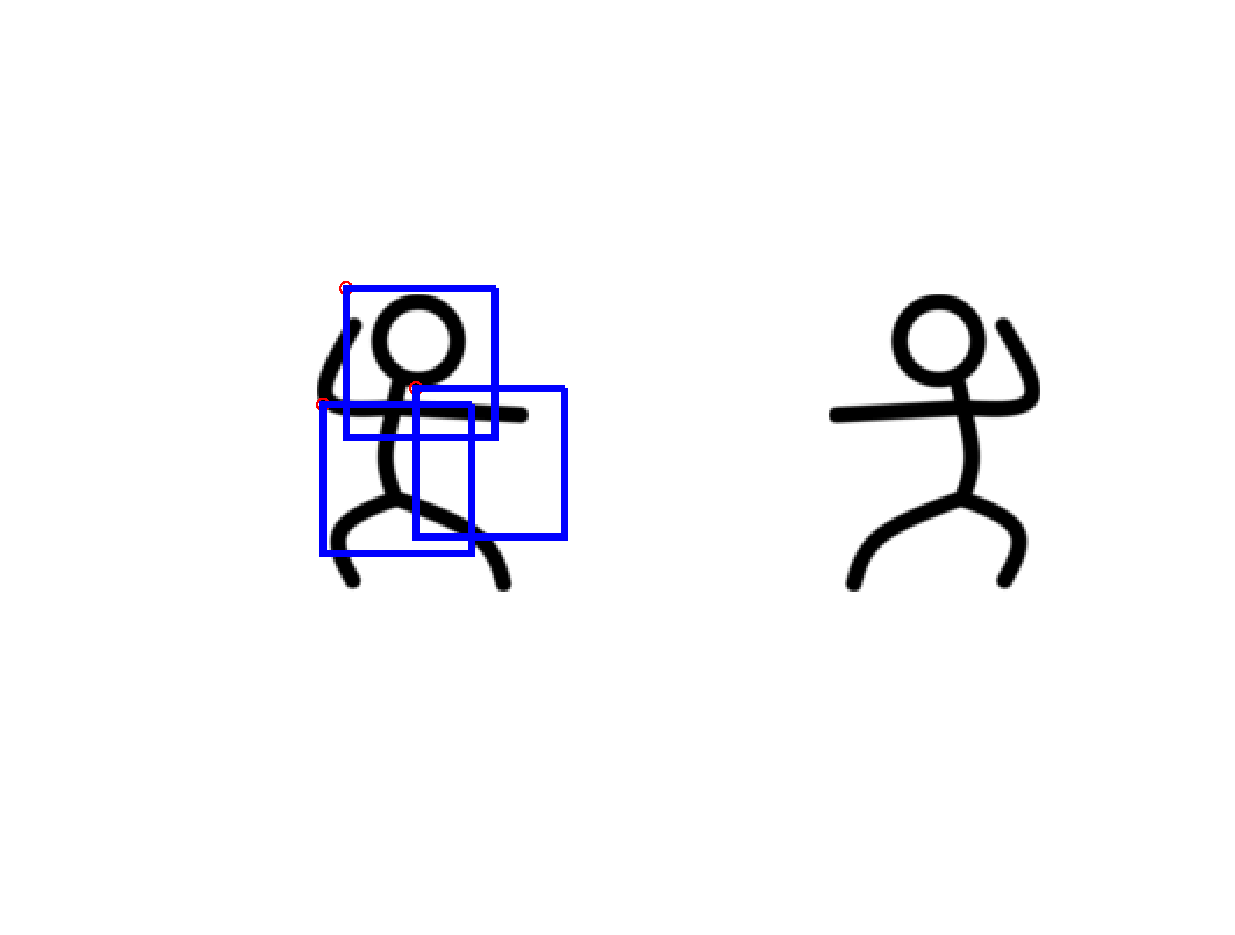
\includegraphics[width=1.0\textwidth]{images/2.eps}
\end{center} 
\end{minipage}%
\begin{minipage}[c]{0.4\textwidth}
\begin{center}
 \textbf{PdsPiv}\\
 Particle image velocimetry
\end{center}
\begin{equation*}
\rho = corr(\mathbf{A},\mathbf{X})
  \end{equation*}
\end{minipage}
\end{frame}
%%%%%%%%%%%%%%%%%%%%%%%%%%%%%%%%%%%%%%%%%%%%%%%%%%%%%%%%%%%%%%%%%%%%%%%%%%%%%%%%%
\begin{frame}{https://sourceforge.net/projects/pdsplibj/}
\begin{center}
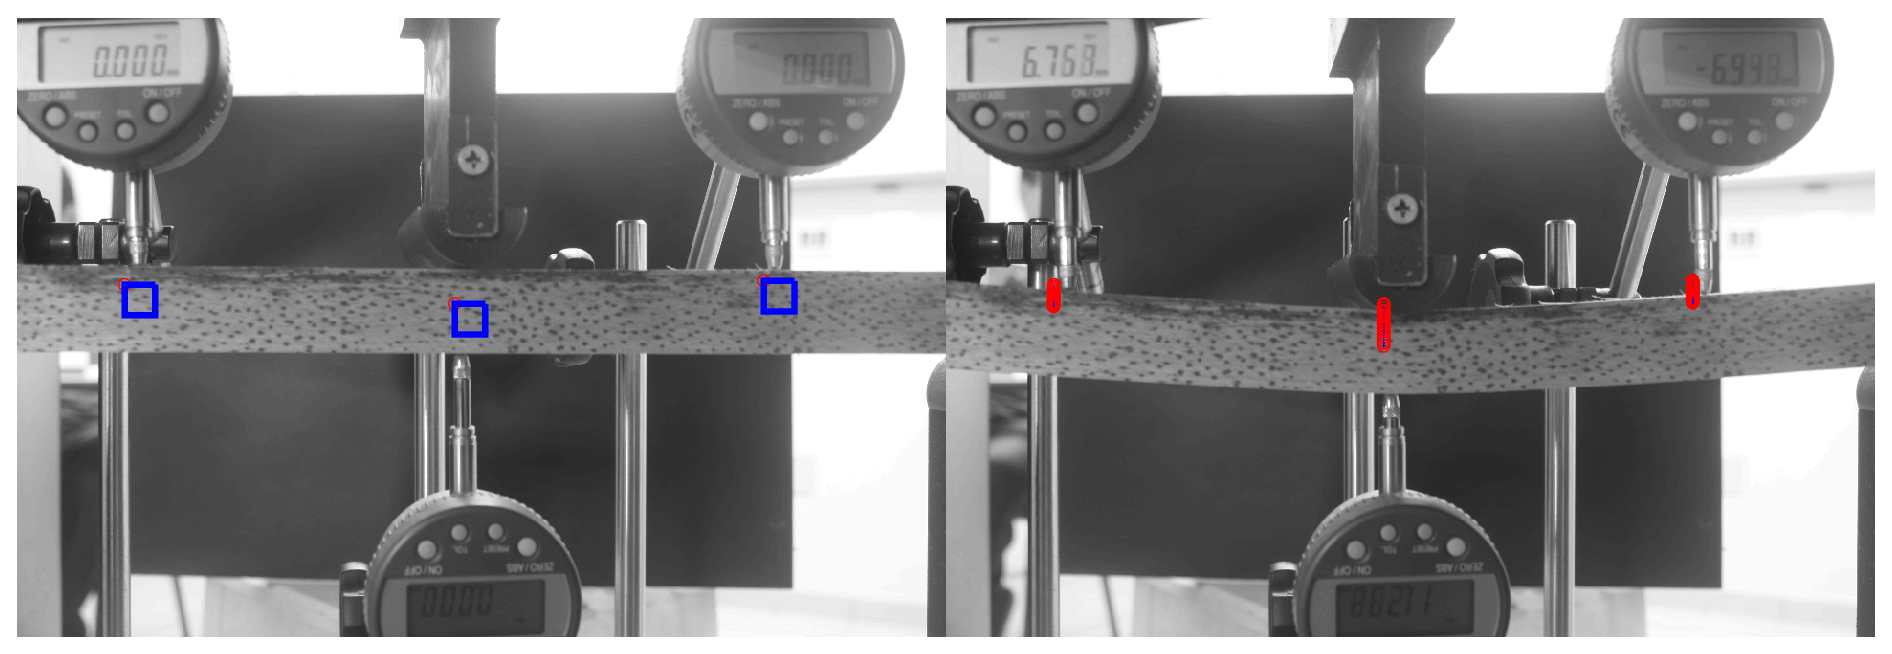
\includegraphics[width=1.0\textwidth]{images/numresult1.eps}
\end{center} 
\end{frame}

%%%%%%%%%%%%%%%%%%%%%%%%%%%%%%%%%%%%%%%%%%%%%%%%%%%%%%%%%%%%%%%%%%%%%%%%%%%%%%%%%
\begin{frame}{https://sourceforge.net/projects/pdsplibj/}
\begin{center}
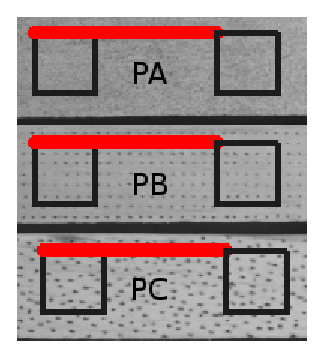
\includegraphics[width=0.55\textwidth]{images/image_px1-64.eps}
\end{center} 
\end{frame}


%%%%%%%%%%%%%%%%%%%%%%%%%%%%%%%%%%%%%%%%%%%%%%%%%%%%%%%%%%%%%%%%%%%%%%%%%%%%%%%%%
\begin{frame}{https://sourcefoge.net/projects/pdsplibj/}
\begin{center}
\begin{figure}
    \centering
    \begin{subfigure}[b]{0.45\textwidth}
        \includegraphics[width=\textwidth]{images/image_plotA-64.eps}
        \caption{Imagem original}
        \label{fig:Tipo A}
    \end{subfigure}
    \begin{subfigure}[b]{0.45\textwidth}
        \includegraphics[width=\textwidth]{images/image_plotB-64.eps}
        \caption{Tipo B}
        \label{fig:image_plotB-64}
    \end{subfigure}
    \begin{subfigure}[b]{0.45\textwidth}
        \includegraphics[width=\textwidth]{images/image_plotC-64.eps}
        \caption{Tipo C}
        \label{fig:image_plotC-64}
    \end{subfigure}
    \begin{subfigure}[b]{0.45\textwidth}
        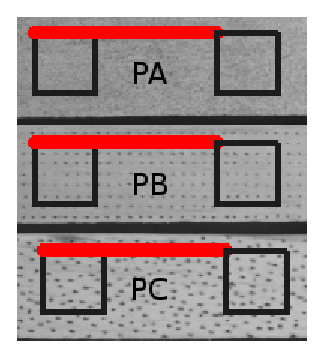
\includegraphics[width=0.5\textwidth]{images/image_px1-64.eps}
        \caption{Tipos de pontos}
        \label{fig:image_px1-64}
    \end{subfigure}
    \caption{PIV analises }\label{fig:PIVtype}
\end{figure}
\end{center} 
\end{frame}


%%%%%%%%%%%%%%%%%%%%%%%%%%%%%%%%%%%%%%%%%%%%%%%%%%%%%%%%%%%%%%%%%%%%%%%%%%%%%%%%
%\begin{frame}[allowframebreaks]
%        \frametitle{References}
%        \bibliographystyle{plain}
%\bibliography{aritmetica}
%\end{frame}



\end{document}
